\section{Comparison Human and GPT4 and GPT4-V}

\begin{figure}[h!t]
\centering
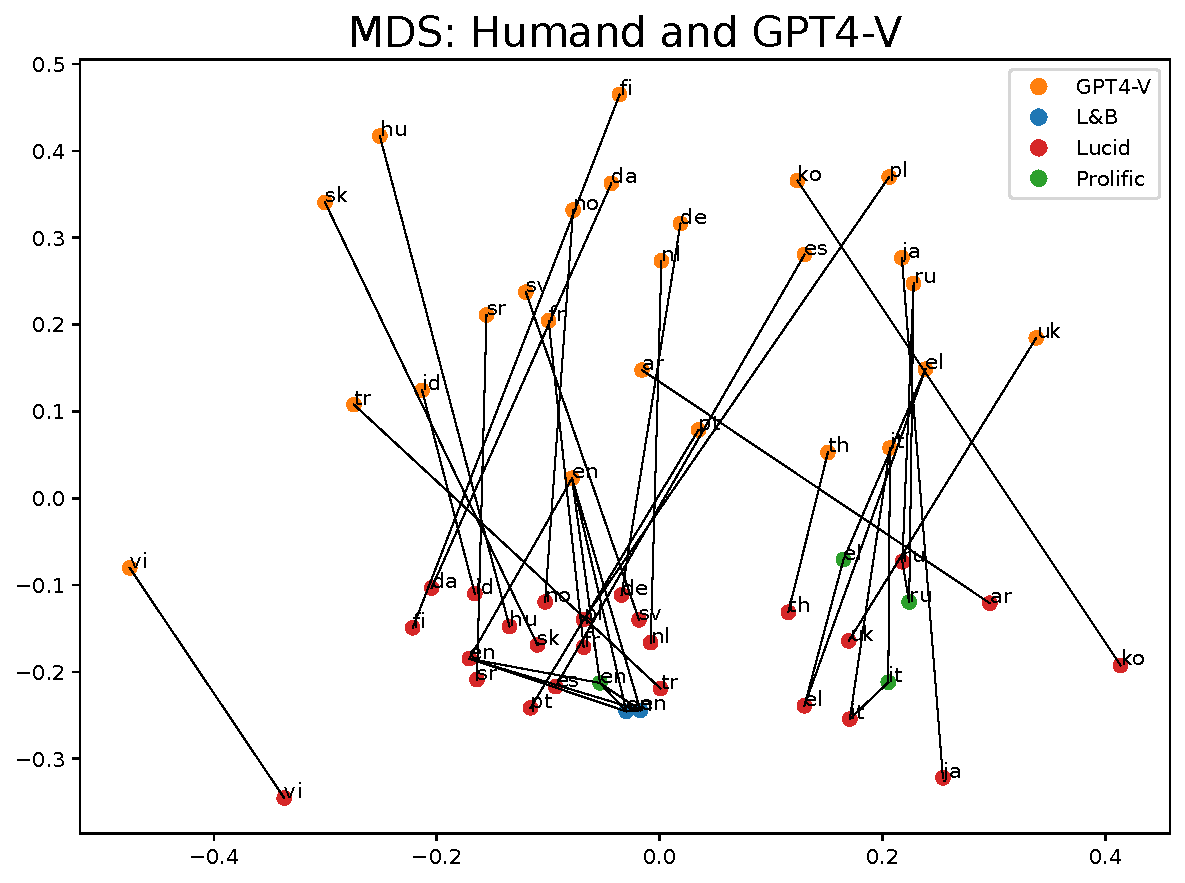
\includegraphics[page=1, width=0.49\linewidth]{images/MDS/mds_rand_index_human_gpt4-v.pdf}
\hfill
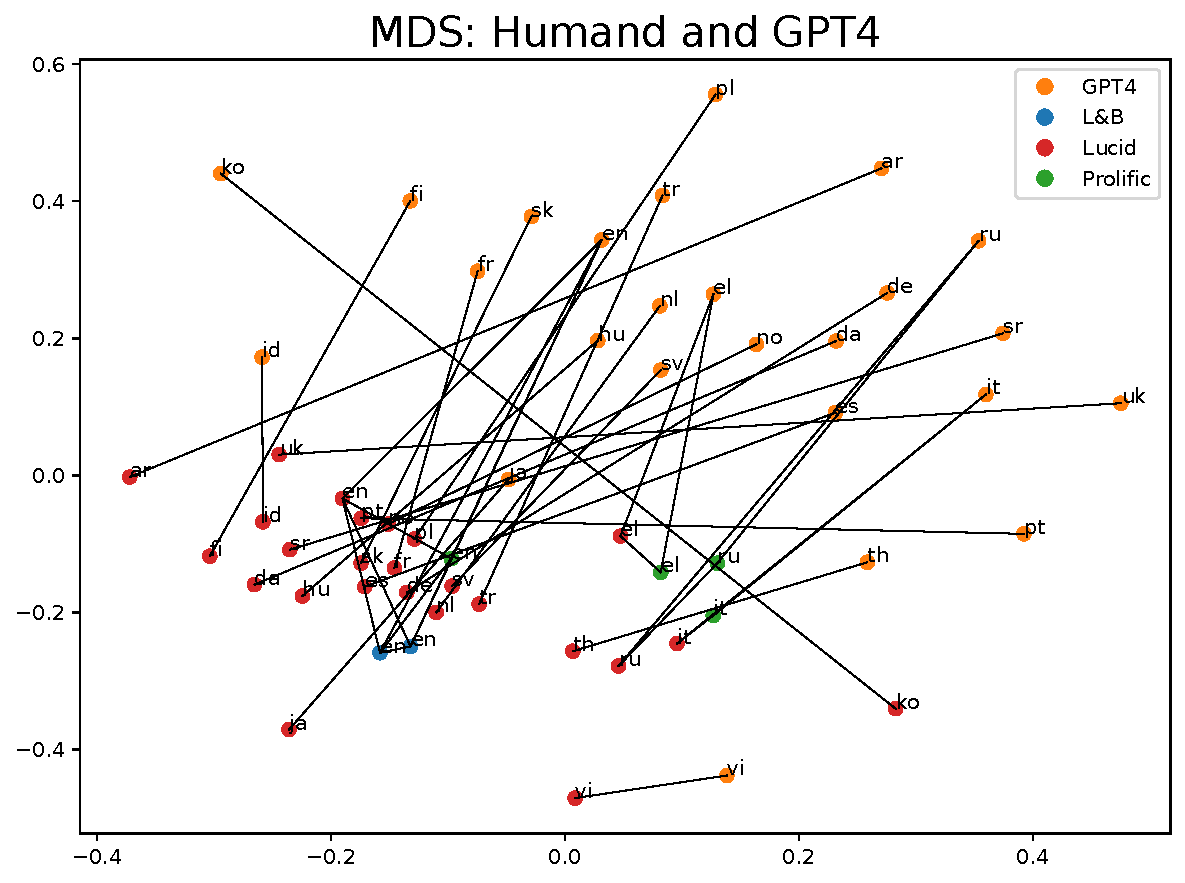
\includegraphics[page=1, width=0.49\linewidth]{images/MDS/mds_rand_index_human_gpt4.pdf}
\decoRule
\caption[MDS ARI Lucid \& GPT4/GPT4-V]{MDS human and GPT4/GPT4-V.
MDS embedding visualizes ARI matrix of human data sets and GPT4-V (left panel) and GPT4 (right panel). To highlight the comparison between different sources identical languages are connected by lines.
The clear division along the y-axis in both panels suggests it acts as a discriminator between human and GPT4 datasets.
The language pairs tend to be aligned along the dividing line which becomes visually apparent with the tendency of the lines to cross the border in a orthogonal way.
Notably, for GPT4-V, language pair positions exhibit a significant correlation which was not reproduced in the human - GPT4 plot(mainly due to outliers like Korean and Arabic.}
\label{fig:MDS_human_gpt}
\end{figure}

To investigate similarities and differences across the human and GPT4 data Fig \ref{fig:MDS_human_gpt} shows an MDS taking a distance matrix calculated from the ARI matrix as input. This MDS differs from the one shown above since we now use both human and GPT4 data. 
The plots make it visually apparent that human and GPT4 or GPT4-V data cover different parts of the MDS space.
However, the corresponding languages seem to be similarly aligned along the dividing border. This gets qualitatively apparent as the connecting lines between the same languages in the two data sets cross the dividing border in a predominantly orthogonal manner. In the GPT4 plot the y-axis is correlated with the position of the languages pairs (r=.45, p=.025; if we exclude the outlier Korean, correlation is even higher: r=.56, p=.004). Visually apparent correlation on the x-axis does not reach significance due to strong outliers like Korean, Arabic and Ukrainian.
For GPT4-V the position of the languages is correlated along the x-axis (r=.67, p < .000). The following can be derived from this: First, the two data sets obtained from humans and GPT4 or GPT4-V are fundamentally different from each other as they group into separate clusters. Second, the correlation of the relative positions of the single languages in the subgroups highlights the preserved similarity across the data sets for single languages.

\begin{figure}[h!t]
\centering
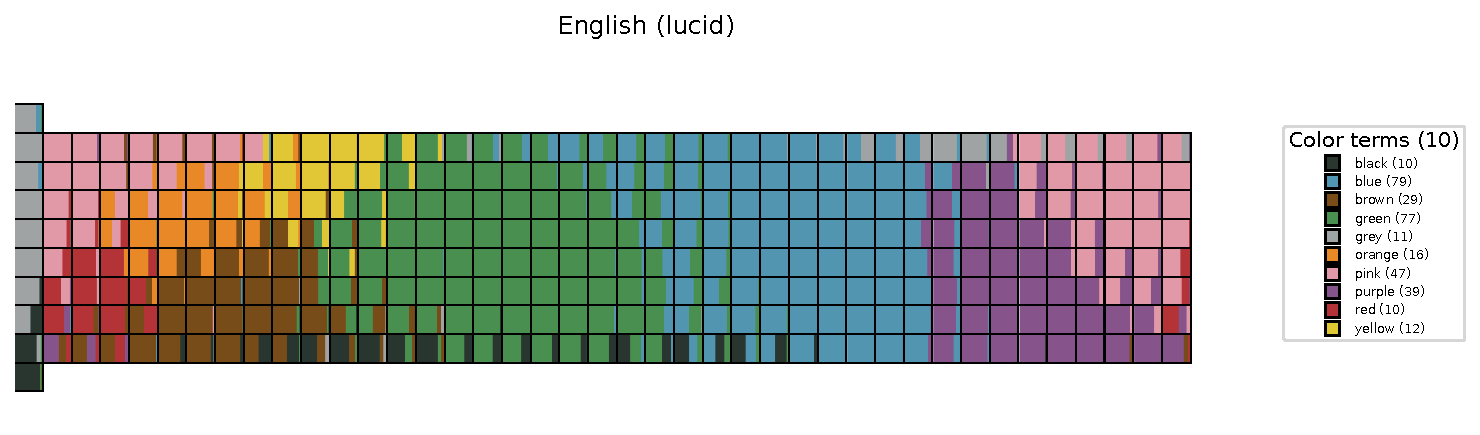
\includegraphics[width=0.49\linewidth]{images/mode_maps/English (lucid).pdf}
\hfill
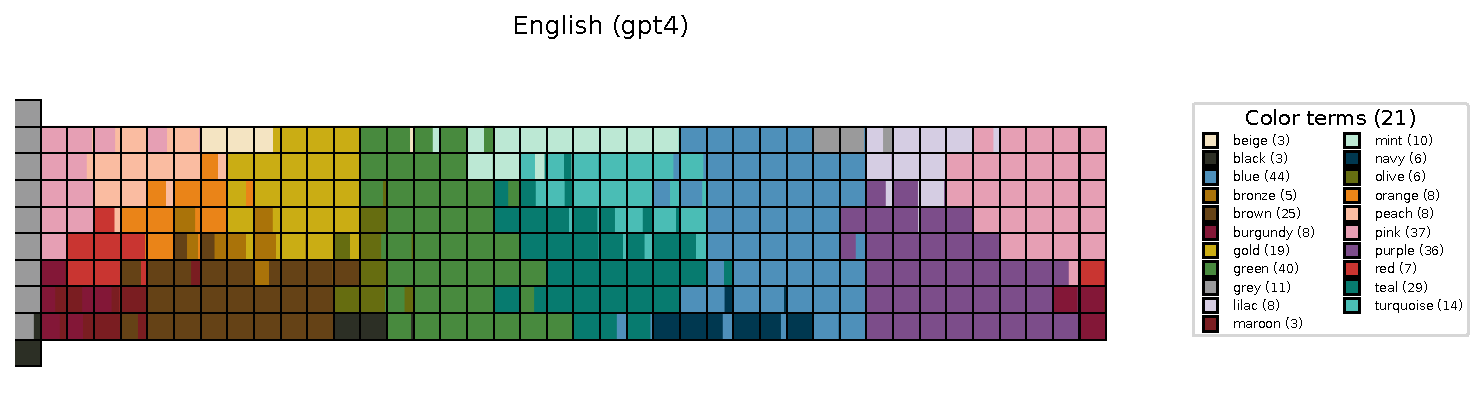
\includegraphics[width=0.49\linewidth]{images/mode_maps_gpt4/English (gpt4).pdf}
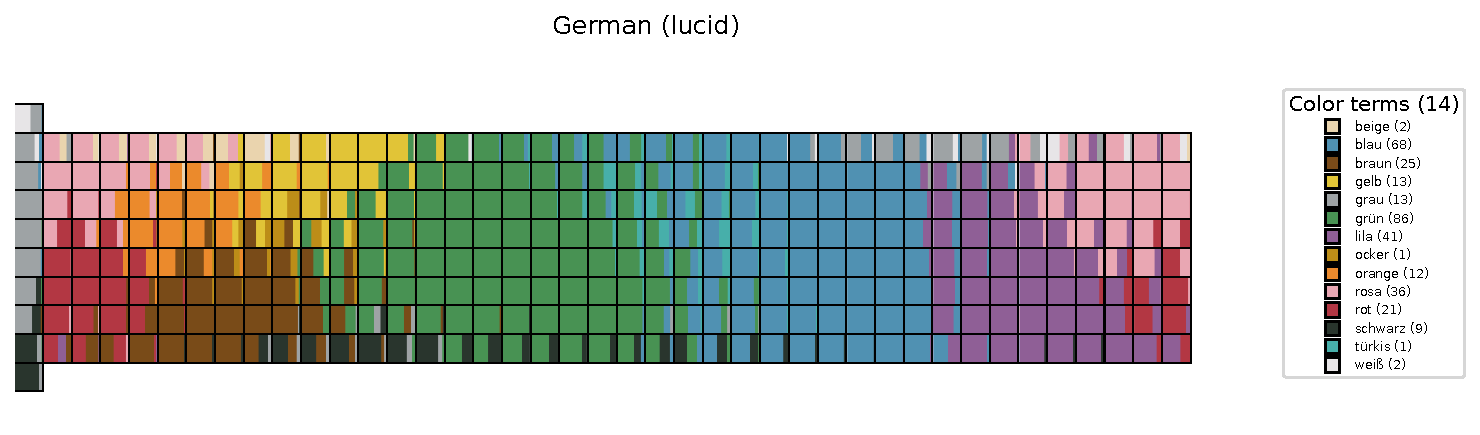
\includegraphics[width=0.49\linewidth]{images/mode_maps/German (lucid).pdf}
\hfill
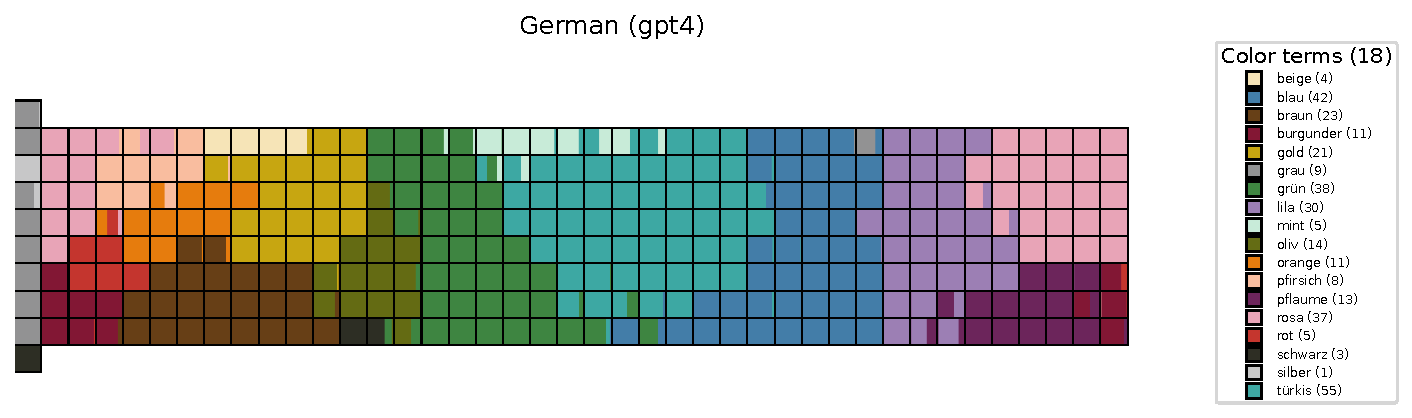
\includegraphics[width=0.49\linewidth]{images/mode_maps_gpt4/German (gpt4).pdf}
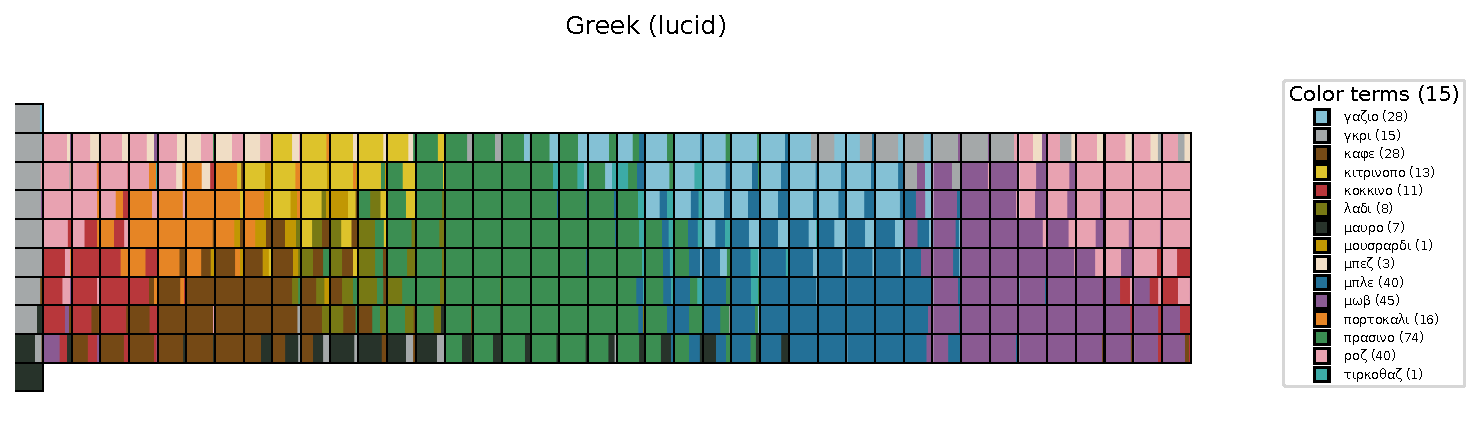
\includegraphics[width=0.49\linewidth]{images/mode_maps/Greek (lucid).pdf}
\hfill
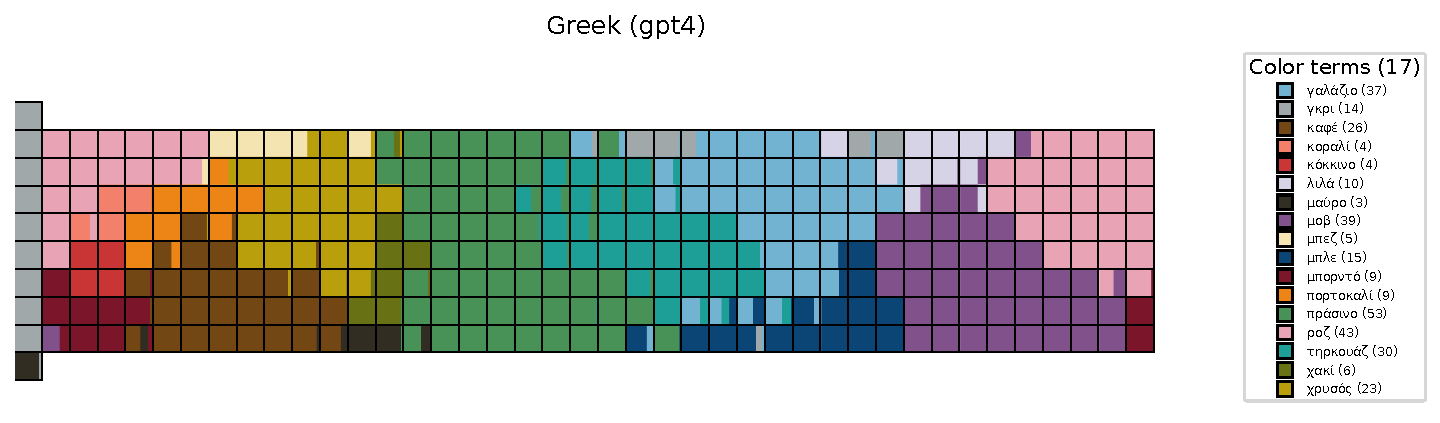
\includegraphics[width=0.49\linewidth]{images/mode_maps_gpt4/Greek (gpt4).pdf}
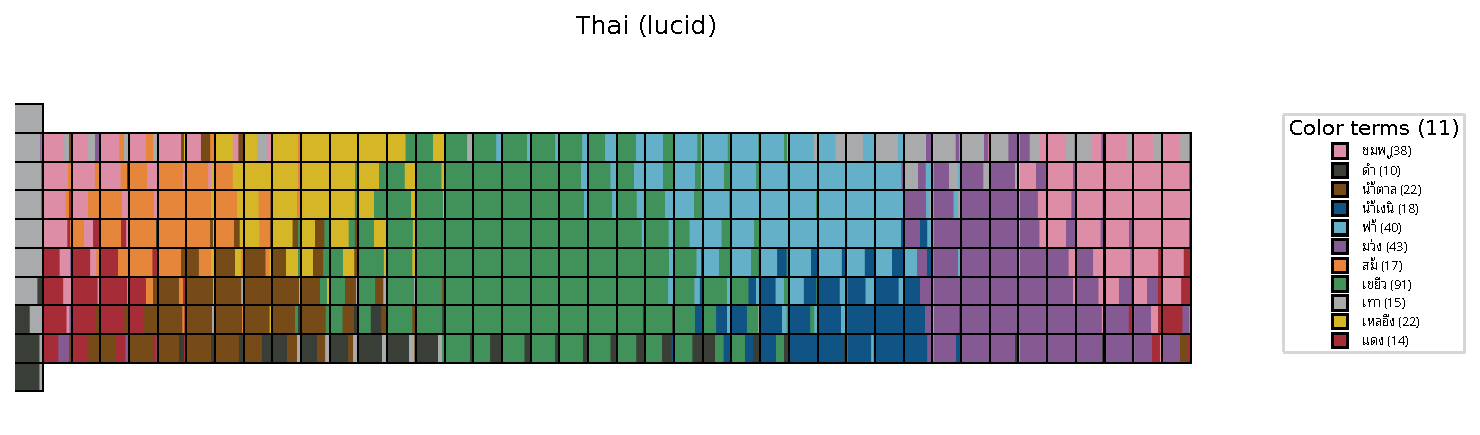
\includegraphics[width=0.49\linewidth]{images/mode_maps/Thai (lucid).pdf}
\hfill
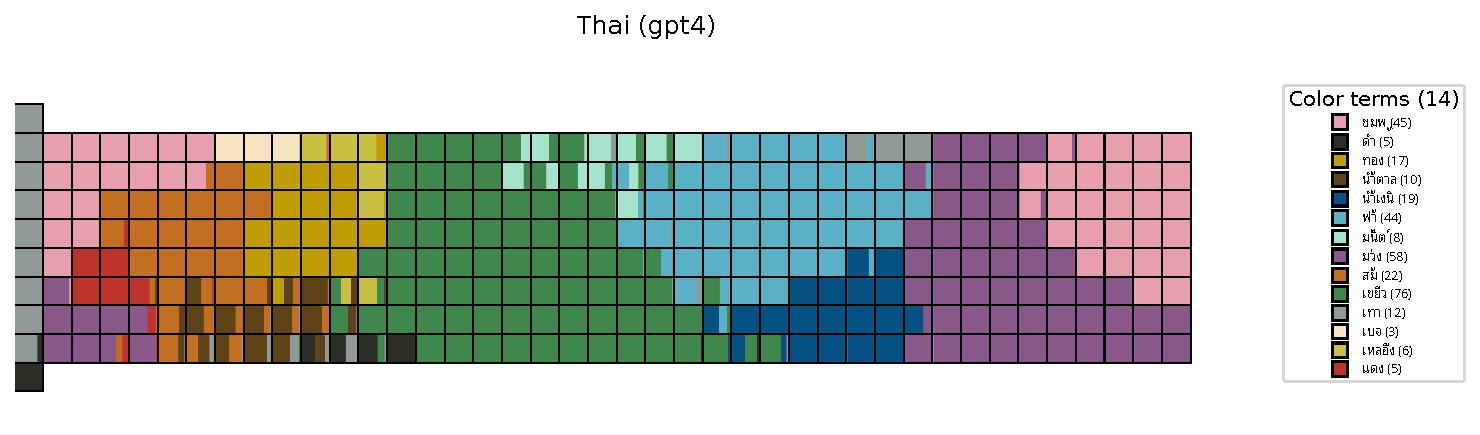
\includegraphics[width=0.49\linewidth]{images/mode_maps_gpt4/Thai (gpt4).pdf}
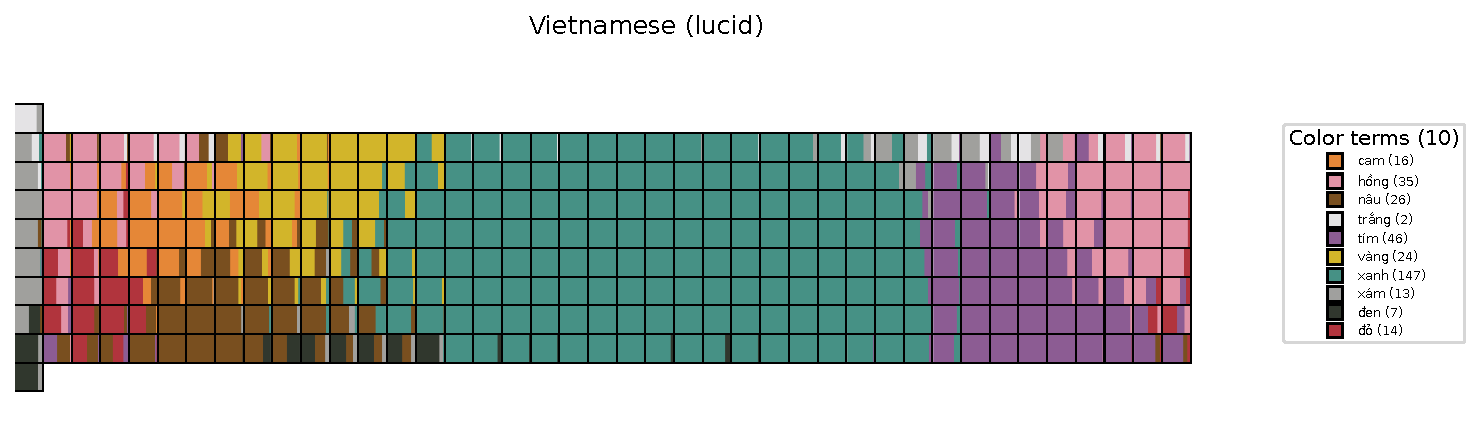
\includegraphics[width=0.49\linewidth]{images/mode_maps/Vietnamese (lucid).pdf}
\hfill
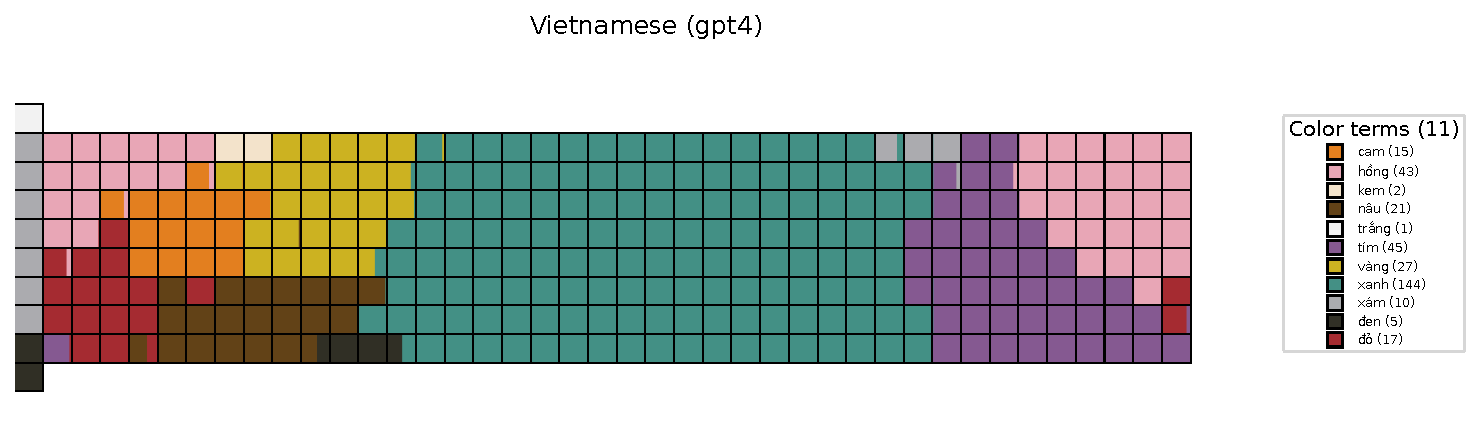
\includegraphics[width=0.49\linewidth]{images/mode_maps_gpt4/Vietnamese (gpt4).pdf}
\caption[Proportion Plots: GPT4 vs Human]{Proportion plots comparing color vocabularies for English, German, Greek, Thai, Vietnamese across human and GPT4 agents.}
\label{fig:mode-maps-human_vs_gpt}
\end{figure}


When qualitatively comparing GPT4 with human proportional plots the GPT4 data exhibit a similar but more detailed naming pattern. 
To compare data of GPT4 and Lucid, Fig. \ref{fig:mode-maps-human_vs_gpt} shows the proportional plots for English, German, Greek, Thai and Vietnamese side by side for both data sets.
Fig \ref{fig:mode-maps-gpt1} and \ref{fig:mode-maps-gpt2} show the full set of proportional plots for all languages elicited from GPT4.
For English the eleven BCT are present in the GPT4 data but subdivided by additional niche categories such as mint, navy, olive, teal and turquoise in the blue and green area. 
Turquoise is a very prominent category throughout most of the GPT4 data, even if the category is small or absent in the Lucid data (English, German, Greek).
Mint is also present in many languages of GPT4 data even if the word is not native to the languages (German, Thai, Danish, Dutch, Polish... E.g. \textthai{มิ้นต์} is the Thai writing for the English word mint and not a native Thai word).
In the case of English this results in a richer color lexicon of eleven additional terms compared to human data (global entropy). 
In Japanese however, GPT4 responds with a lower number of color terms. Especially, \japaneseText{ミズ色} the light blue category is absent.
The plots also illustrate low entropy in the responses for each chip (local entropy). Compared to human data, the individual chips show fewer different colors, reflecting a more uniform way of responding.
However, the comparison also reveals a tendency that languages such as Vietnamese which have a small color vocabulary in the human data also have fewer color terms listed for the GPT4 data. In contrast languages like German and Greek with larger color vocabularies also have higher numbers of color terms in the respective GPT4 Data.


\begin{figure}[h!t]
\centering
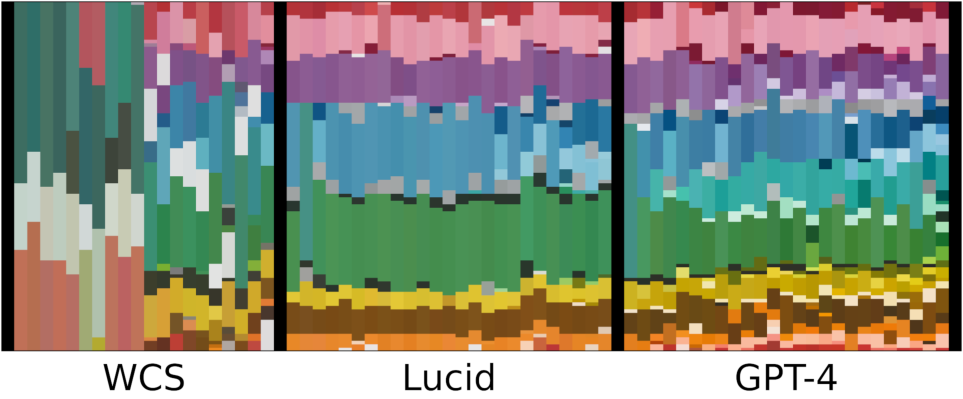
\includegraphics[page=1, width=\linewidth]{images/stream_plot.pdf}
\decoRule
\caption[Stream Plot]{Color Category Differentiation Across WCS, Lucid, and GPT4 Data Sets. This stream plot visualizes the evolution of color category vocabularies across WCS, Lucid, and GPT4 data sets, aligning languages by the number of color categories used, from those with fewer categories (left) to those with many (right). Specifically, for the WCS data set, only the 10 languages with the lowest and highest numbers of color terms are illustrated. This showcases a progression from languages utilizing as few as three color terms, similar to those observed in the WCS data set, to the more complex lexicons found in Lucid data. Remarkably, GPT4 data display a pronounced trend towards the segmentation of color space into very fine categories, exemplified by the emergence of turquoise as a distinct major color category.}
\label{fig:stream_plot}
\end{figure}

Fig \ref{fig:stream_plot} illustrates the number of color terms per collected language divided into the three examined data sets (For simplicity the GPT4-V data are not presented).
For the 110 languages in the WCS dataset the 20 languages with the lowest and highest number of color terms are depicted.
This visualization gives an intuitive understanding in how the three data sets differ. The WCS includes languages of very few color terms, essentially differentiating between warm, cold and light. It also contains languages with higher numbers of color terms overlapping in the number and size of the color categories in the collected data on Lucid. 
The GPT4 Data however show a growing differentiation far beyond the Lucid data.



\begin{figure}[h!t]
\centering
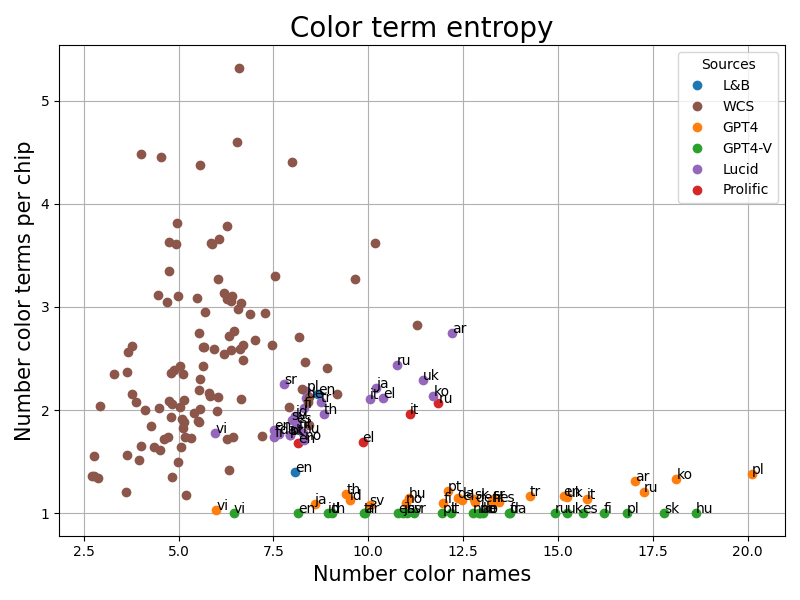
\includegraphics[page=1, width=\linewidth]{images/MDS/entropy-plot.png}
\decoRule
\caption[Entropy Plot]{Entropy Plot: Number of color terms for single chips (exp of local entropy) compared to number of color terms overall (exp. of global entropy) for WCS, Lucid, Prolific, GPT4, and GPT4-V.
GPT4 and GPT4-V exhibit relatively large color lexica and deterministic response behavior (Low local entropy in GPT4-V because of procedure).
Local entropy of human data (Lucid, Prolific, WCS, L\%B) is consistently higher and overlaps across data sets. 
Compared to the WCS, the other human datasets containing data from industrialized languages have larger color vocabularies. This supports \textcite{gibsonColor2017}'s hypothesis that industrialization may drive the development of new color terms.}
\label{fig:entropy_plot}
\end{figure}

Thus global vs. local entropy might drive the differences we see in the mixed MDS plots from above. This relationship is investigated on Fig \ref{fig:entropy_plot} which plots local entropy on the y-axis vs. global entropy on the x-axis. Global entropy here means the number of color terms computed as the exponent of the entropy on all chips.
Again we see distinct clusters for the data of the WCS, the newly collected data, GPT4 and GPT4-V.
The human data sets are adjacent but differ in the number of mean color terms significantly. As reported earlier the WCS languages cover a significant small number of color terms on average. The variance in both data sets are equally high (WCS=1.60, Lucid=1.58).
However, across all data sets the WCS data show the highest local entropy and therefore lowest consensus.

In contrast, the GPT4 data shows a more deterministic character. GPT4 and GPT4-V use significantly less diverse color names per chip compared to the collected human data ( p<.001 for both cases via Wilcoxon-Rank test).
The opposite effect can be observed for the total number of color term. The color lexicon of the GPT4 and GPT4-V data are significantly larger than for the human data ( p<.001 for both cases via Wilcoxon-Rank test).

\begin{figure}[h!t]
\centering
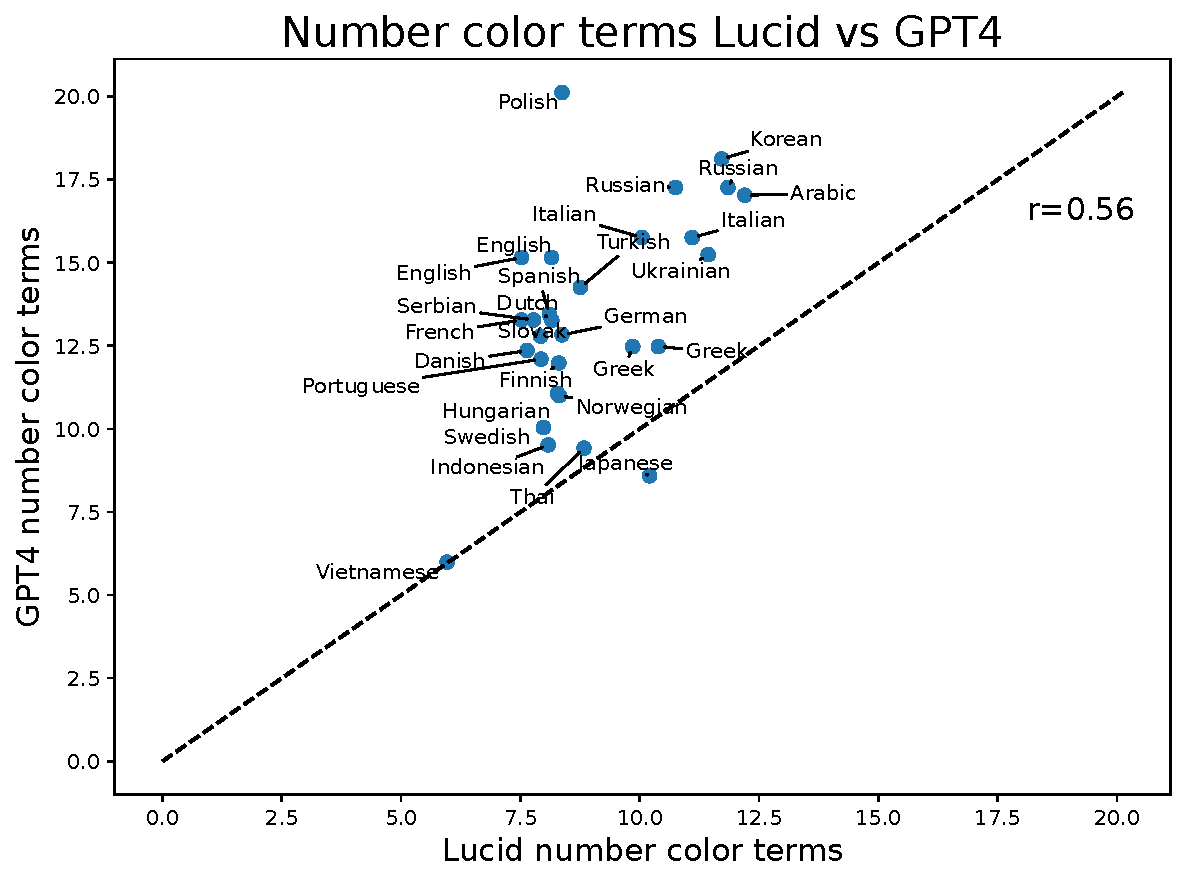
\includegraphics[page=1, width=\linewidth]{images/human_vs_gpt4.pdf}
\decoRule
\caption[Number of color terms]{Number of color terms across languages for Lucid and GPT4. Data indicate larger color vocabularies for GPT4 compared to Lucid data (except Japanese). However, the number of color terms is correlated across languages, proposing that languages with few color terms in Lucid data tend to have a smaller number of color terms in GPT as well.}
\label{fig:human_vs_gpt4}
\end{figure}

However, we see that the number of color categories tend to be strongly correlated across languages for GPT4 and humans (r=.56, p=.002, Fig. \ref{fig:human_vs_gpt4}) but rather weak across GPT4-V and humans (r=.14, p=.479). This indicates that languages with a small number of categories in humans (such as Vietnamese) also tend to have fewer categories in GPT4 and vice versa.
Japanese is one exception here. As mentioned earlier the GPT4 data do not even include the major light blue category. 

Moreover, high correlation of the global entropy with the y-axis in Fig. \ref{fig:MDS_human_gpt} was found for Lucid - GPT4 and Lucid - GPT4-V (r=.79, p<.000, r=.78, p<.000) highlighting that the difference between the two respective data sets are mainly based on the global entropy. 
For the x-axis correlation was lower but still significant (r=.51, p<.000, r=.32, p<.015).

\begin{figure}[h!t]
\centering
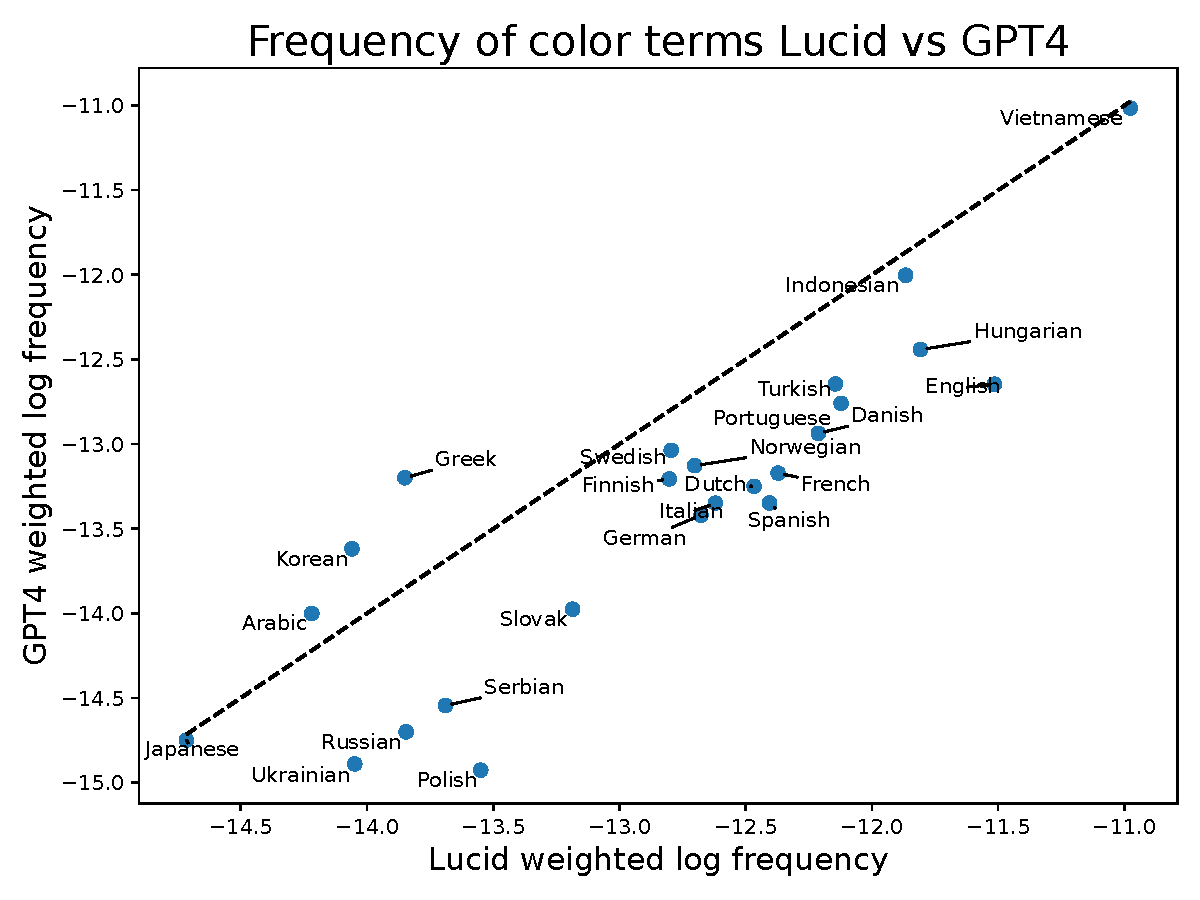
\includegraphics[page=1, width=\linewidth]{images/frequency_plot.pdf}
\decoRule
\caption[Frequency of Color terms]{Logarithmic mean frequency of color terms across languages comparing human data with GPT4 output. The data suggest that GPT4 uses color terms that are less commonly used in the respective languages.}
\label{fig:frequency_plot}
\end{figure}

A further examination of the list of color terms across human and GPT4 data showed a higher usage of infrequently used color terms in the respective languages for GPT4 (Fig. \ref{fig:frequency_plot}).
Apart from Arabic, Korean and Greek GPT4 employ overall less frequently used color terms. This might be related to the specific scripts they used. Compared to the other languages the cleaning heuristics apply fundamental changes in these cases such as the conversion into another script. This might case that the single terms might be less efficiently mapped to words in the respective language.
Whereas the distinction between GPT4 and human is almost significant (p=.059, via the Mann-Whitney U test) the relation is still highly correlated (r=.87, p<.000).


\begin{figure}[h!t]
\centering
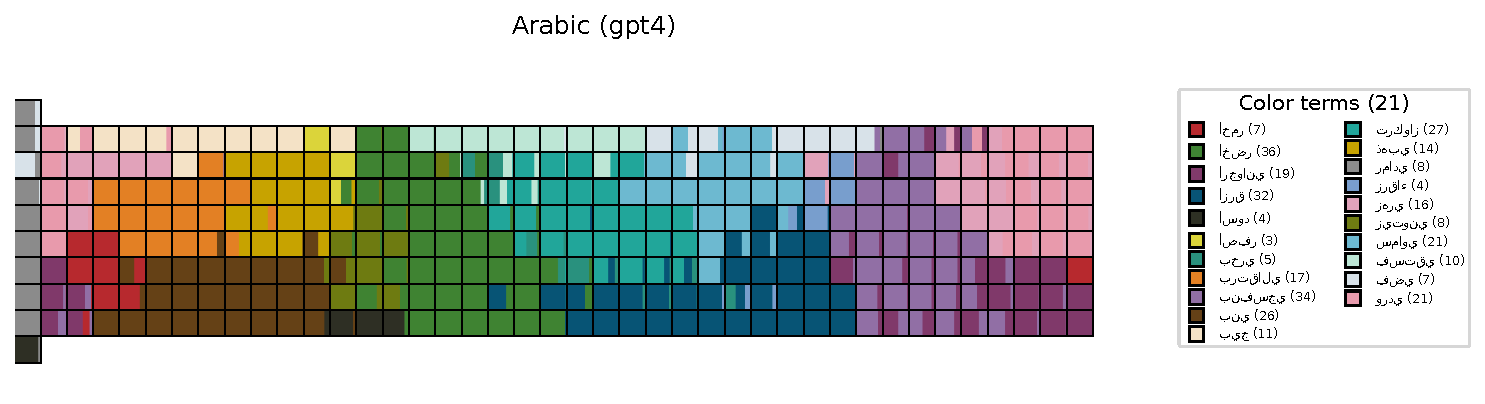
\includegraphics[width=0.49\linewidth]{images/mode_maps_gpt4/Arabic (gpt4).pdf}
\hfill
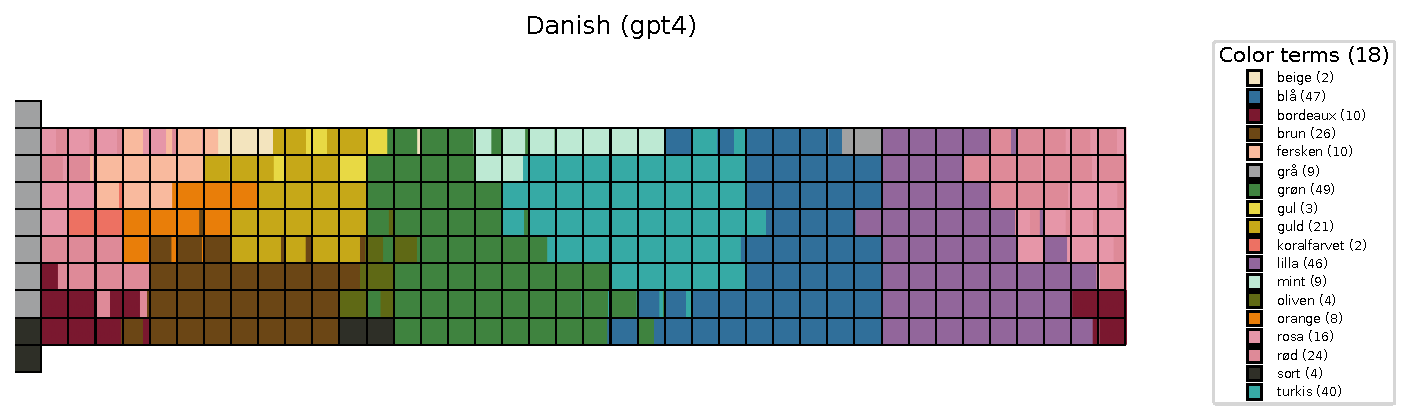
\includegraphics[width=0.49\linewidth]{images/mode_maps_gpt4/Danish (gpt4).pdf}
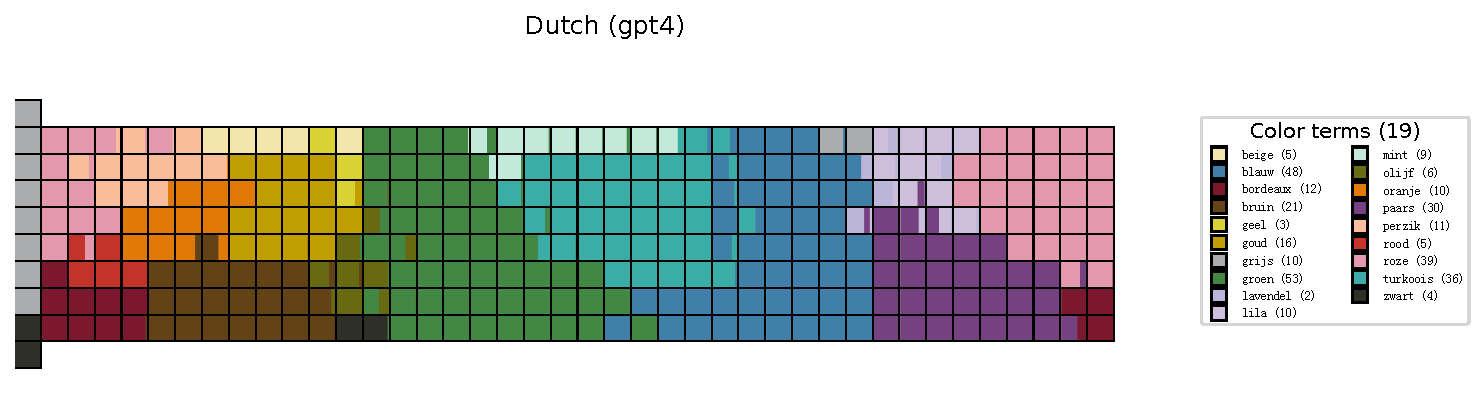
\includegraphics[width=0.49\linewidth]{images/mode_maps_gpt4/Dutch (gpt4).pdf}
\hfill
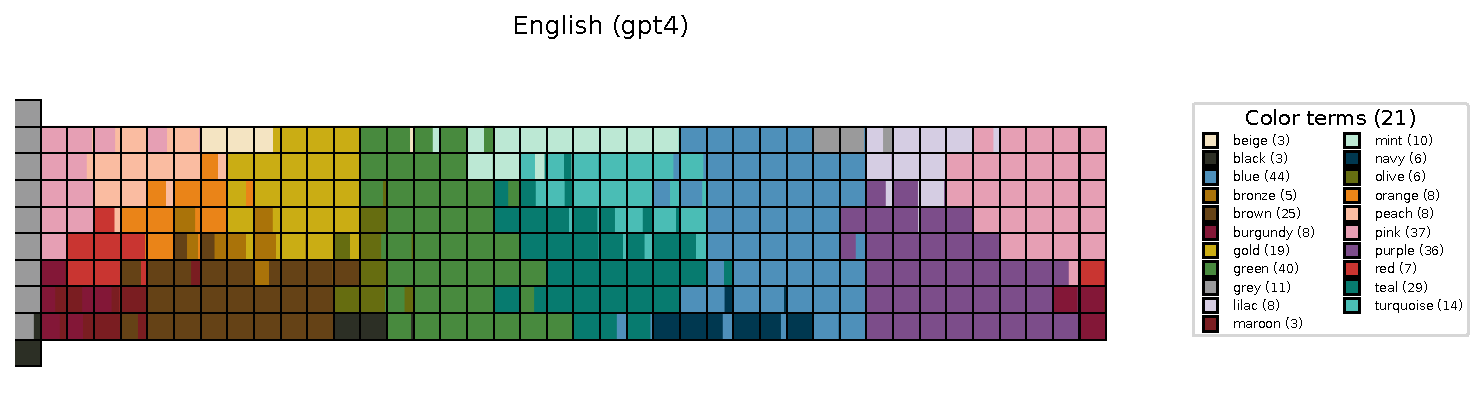
\includegraphics[width=0.49\linewidth]{images/mode_maps_gpt4/English (gpt4).pdf}
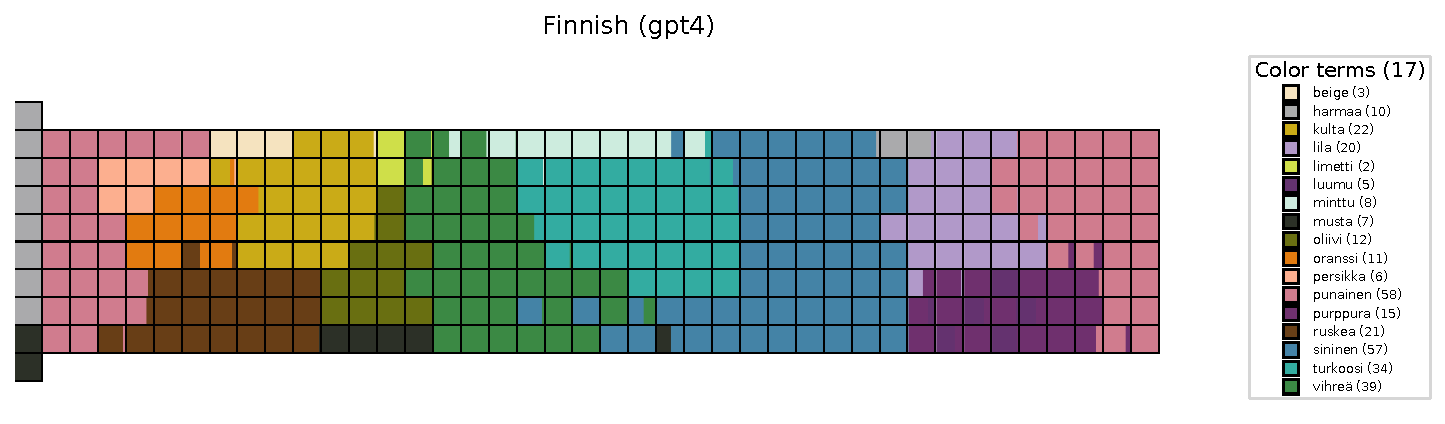
\includegraphics[width=0.49\linewidth]{images/mode_maps_gpt4/Finnish (gpt4).pdf}\hfill
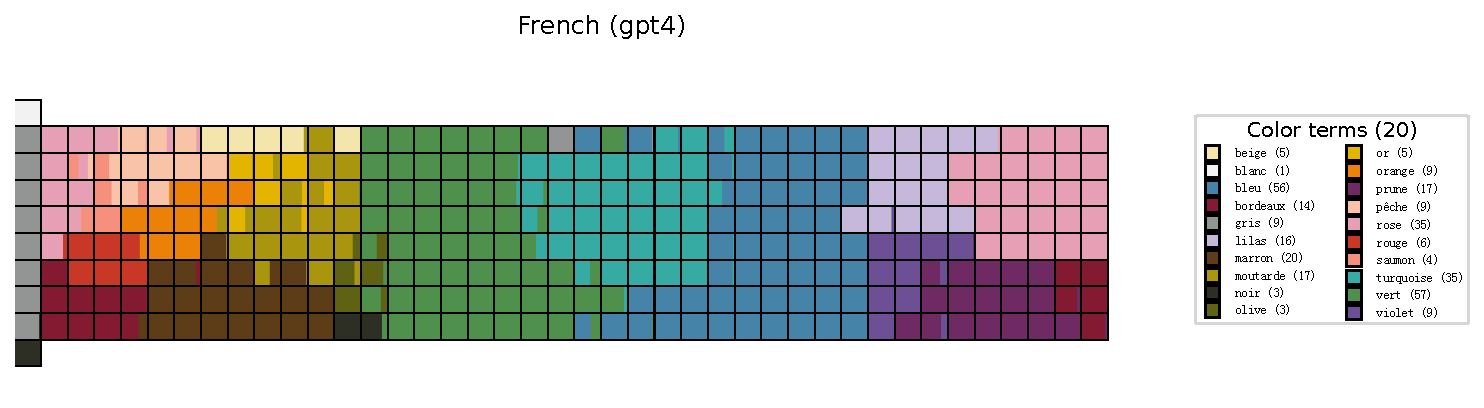
\includegraphics[width=0.49\linewidth]{images/mode_maps_gpt4/French (gpt4).pdf}
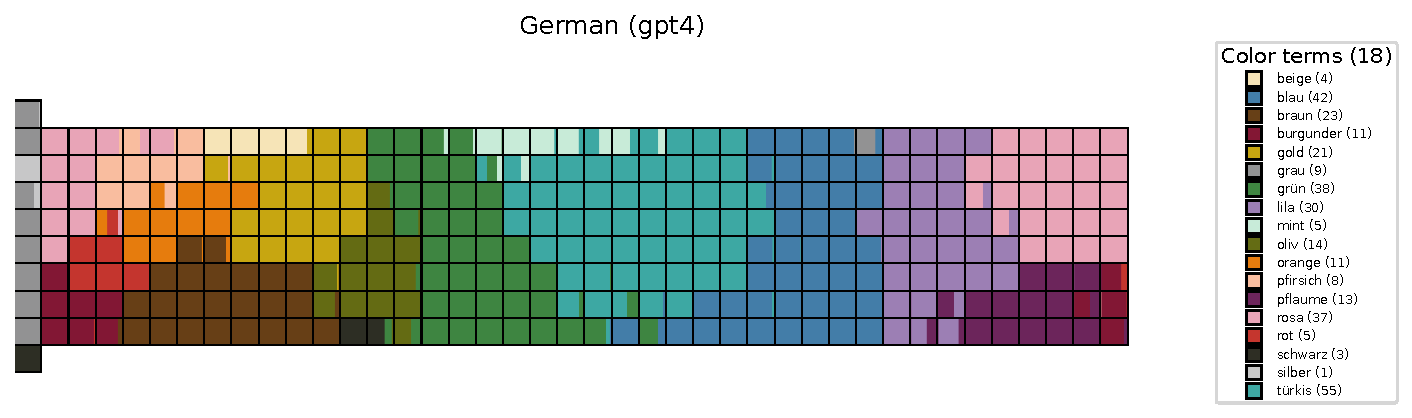
\includegraphics[width=0.49\linewidth]{images/mode_maps_gpt4/German (gpt4).pdf}\hfill
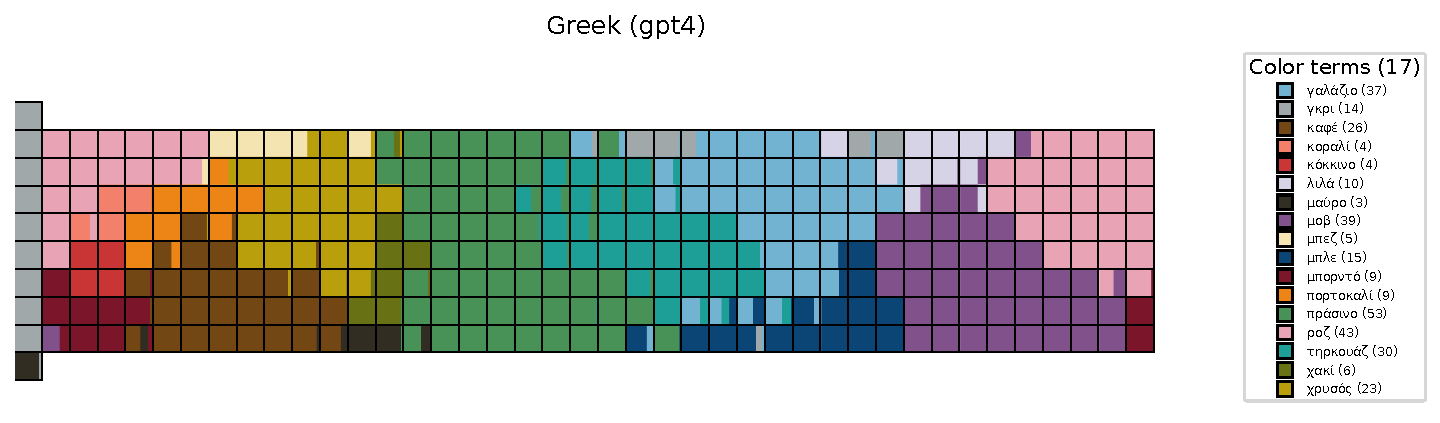
\includegraphics[width=0.49\linewidth]{images/mode_maps_gpt4/Greek (gpt4).pdf}
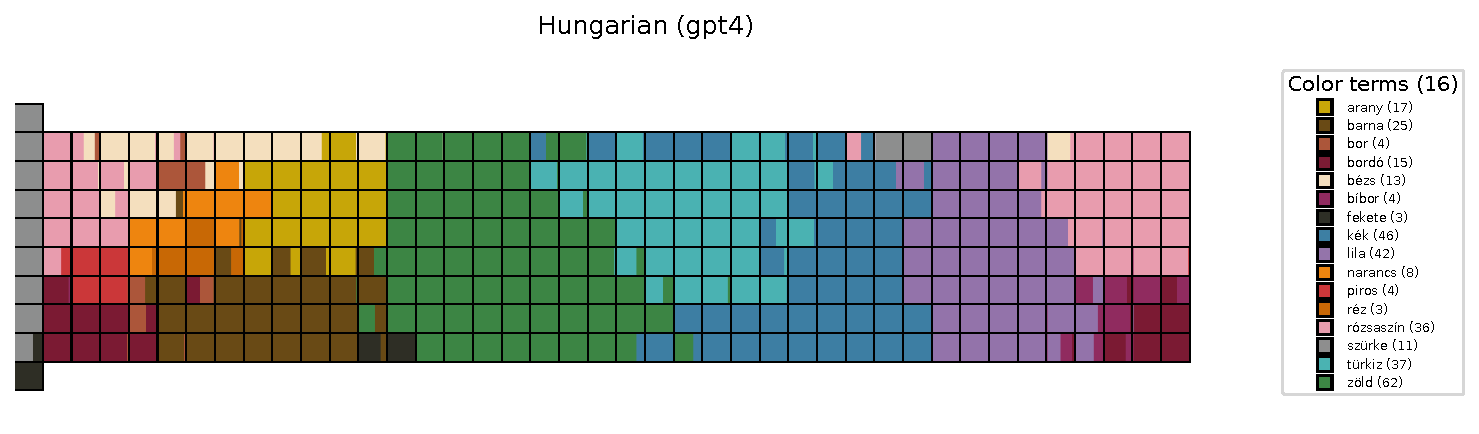
\includegraphics[width=0.49\linewidth]{images/mode_maps_gpt4/Hungarian (gpt4).pdf}
\hfill
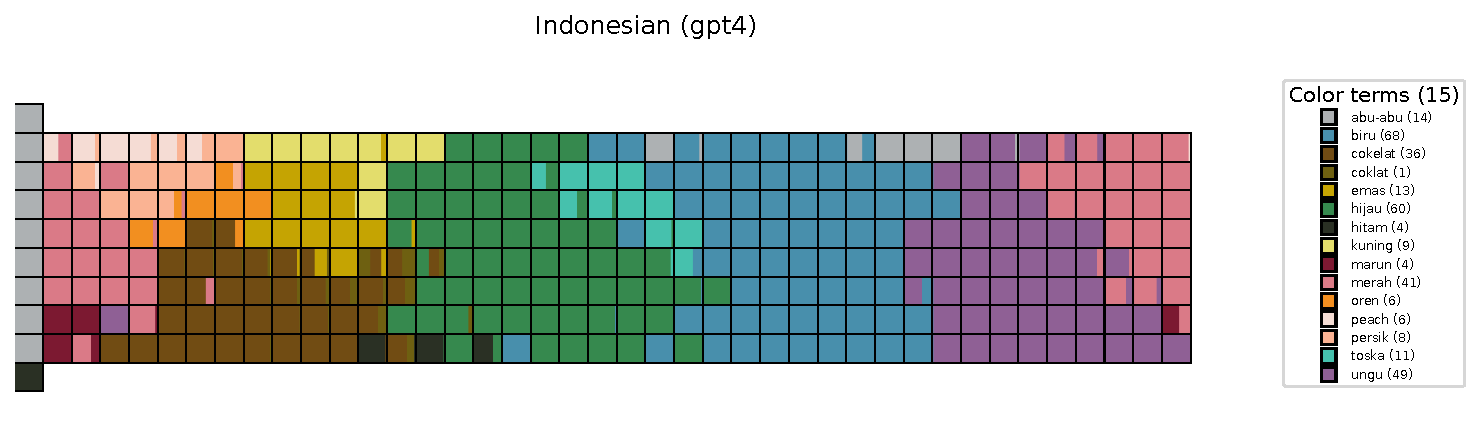
\includegraphics[width=0.49\linewidth]{images/mode_maps_gpt4/Indonesian (gpt4).pdf}
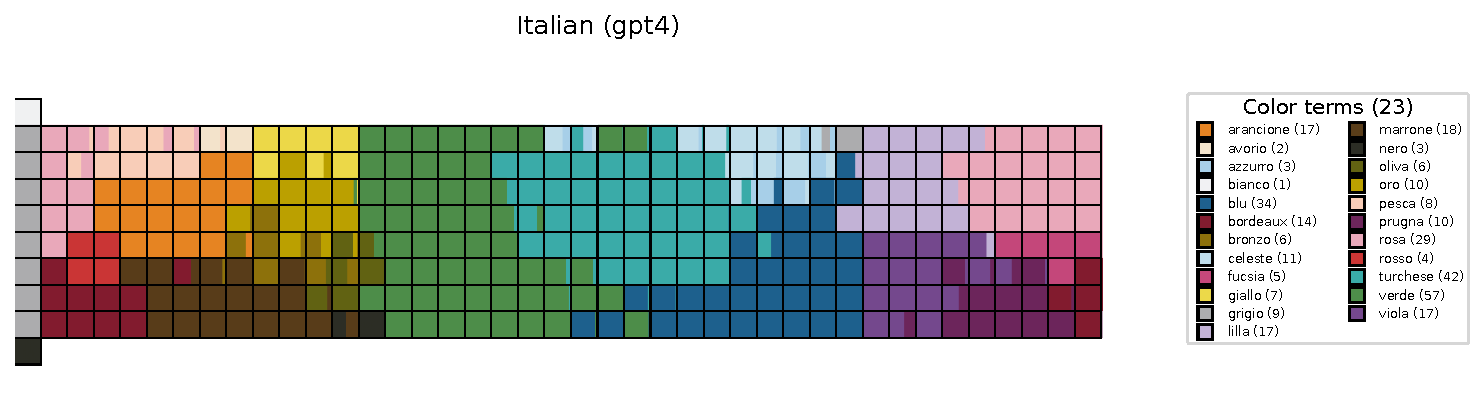
\includegraphics[width=0.49\linewidth]{images/mode_maps_gpt4/Italian (gpt4).pdf}
\hfill
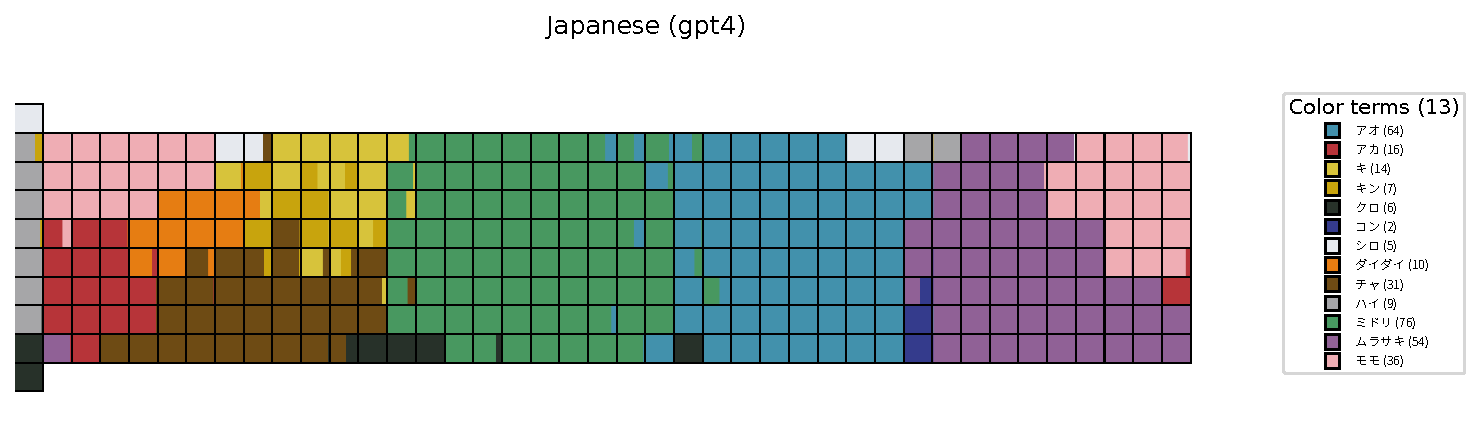
\includegraphics[width=0.49\linewidth]{images/mode_maps_gpt4/Japanese (gpt4).pdf}
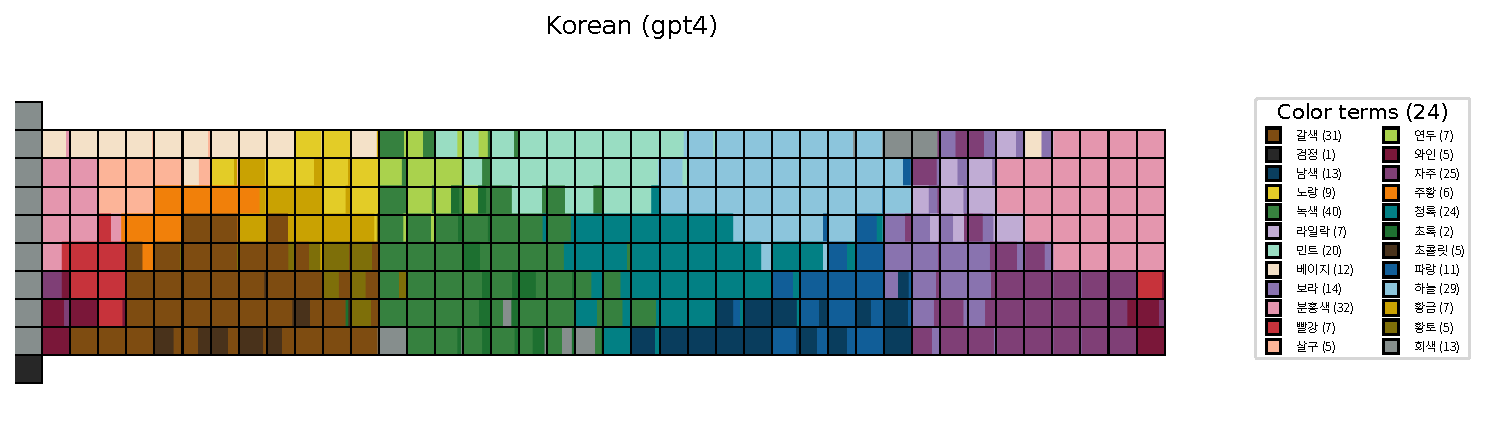
\includegraphics[width=0.49\linewidth]{images/mode_maps_gpt4/Korean (gpt4).pdf}
\hfill
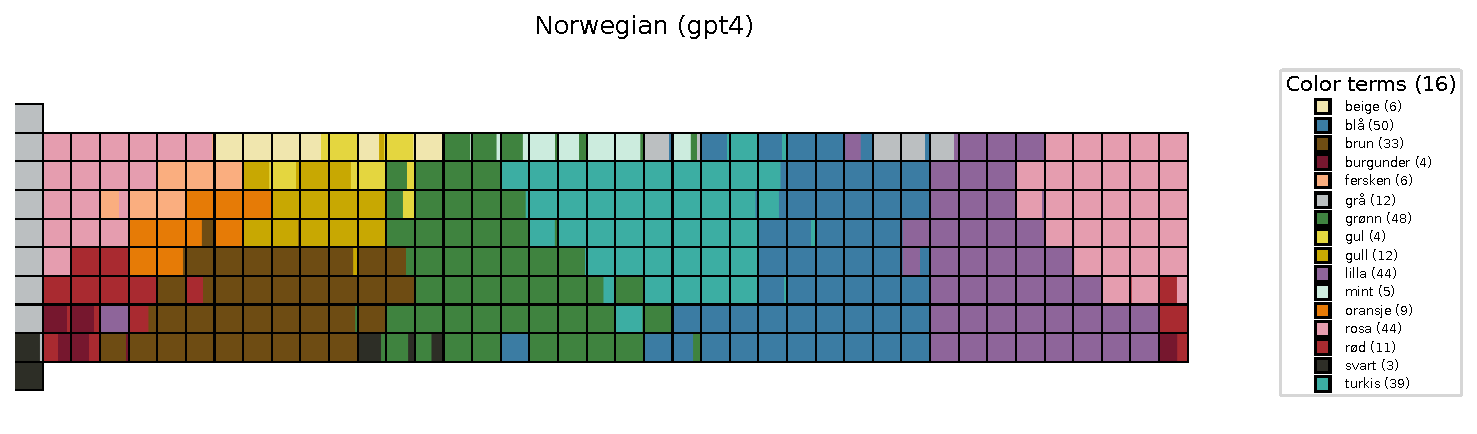
\includegraphics[width=0.49\linewidth]{images/mode_maps_gpt4/Norwegian (gpt4).pdf}
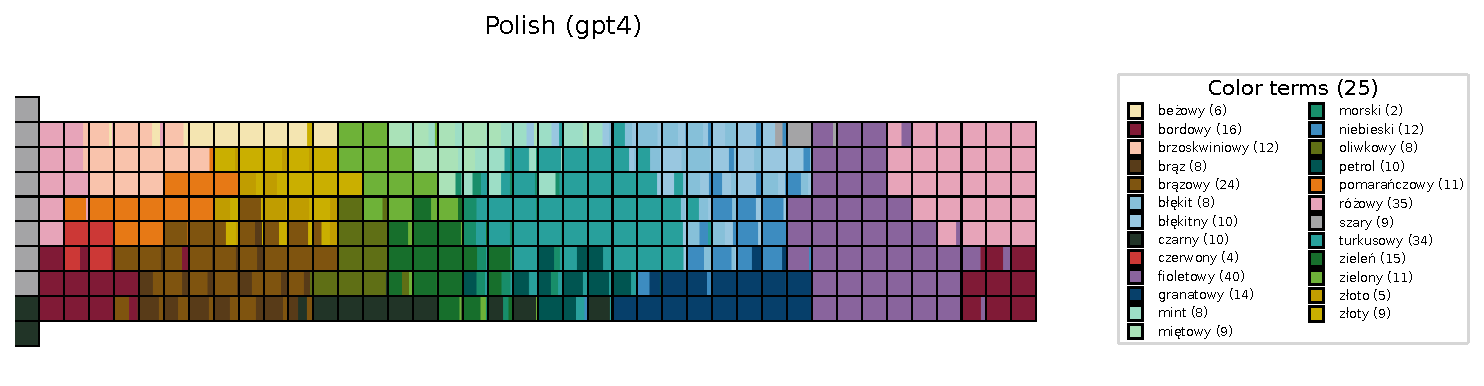
\includegraphics[width=0.49\linewidth]{images/mode_maps_gpt4/Polish (gpt4).pdf}
\hfill
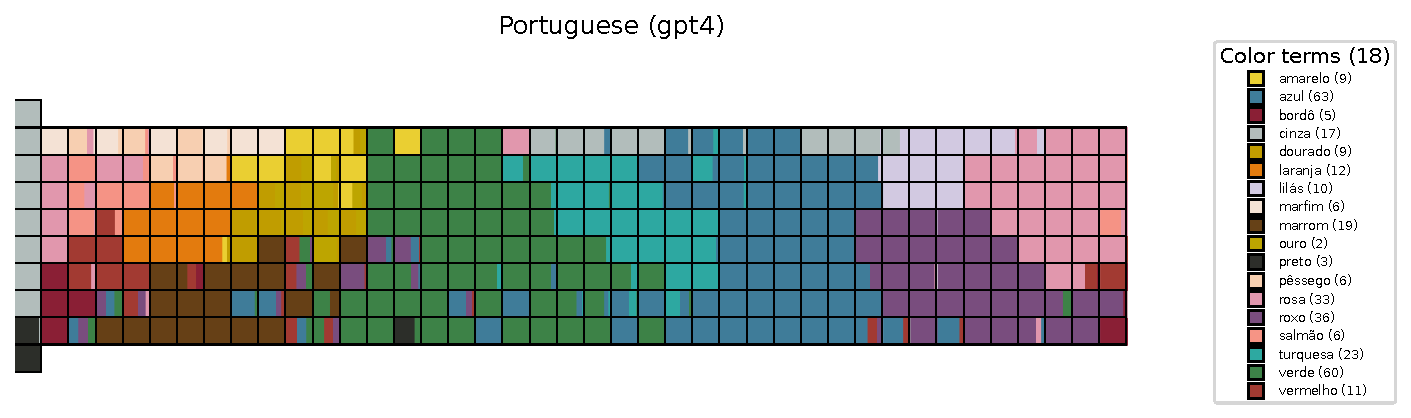
\includegraphics[width=0.49\linewidth]{images/mode_maps_gpt4/Portuguese (gpt4).pdf}
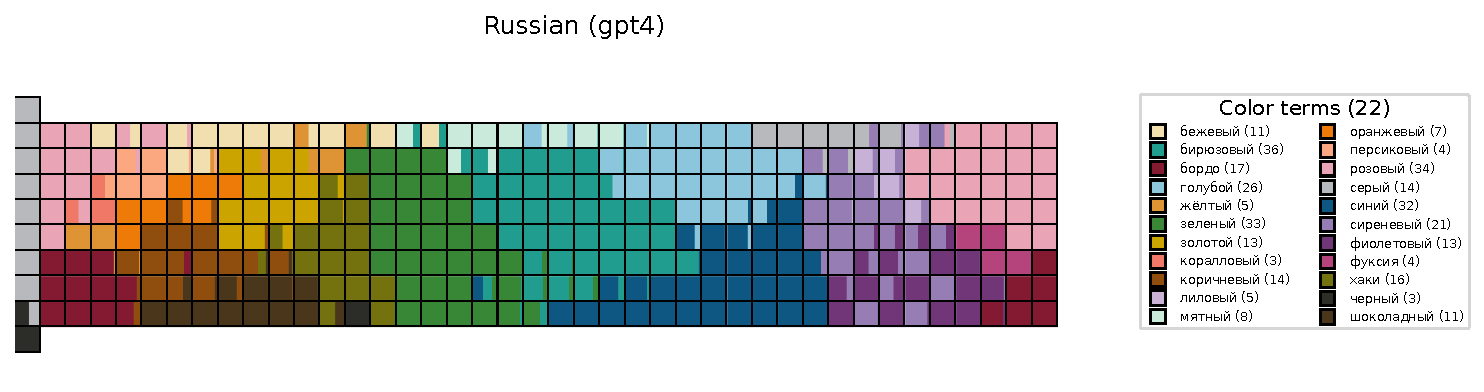
\includegraphics[width=0.49\linewidth]{images/mode_maps_gpt4/Russian (gpt4).pdf}
\hfill
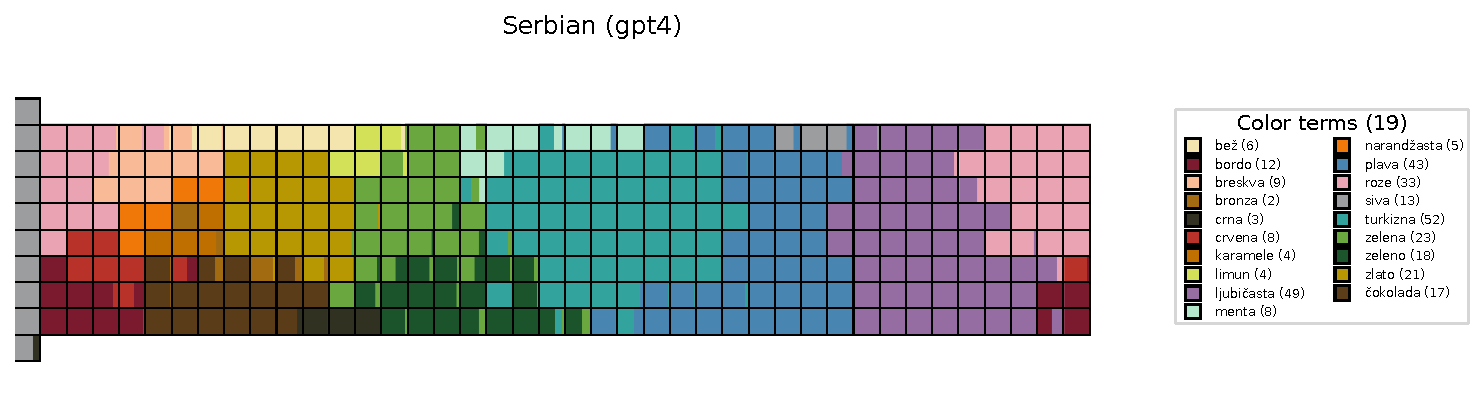
\includegraphics[width=0.49\linewidth]{images/mode_maps_gpt4/Serbian (gpt4).pdf}
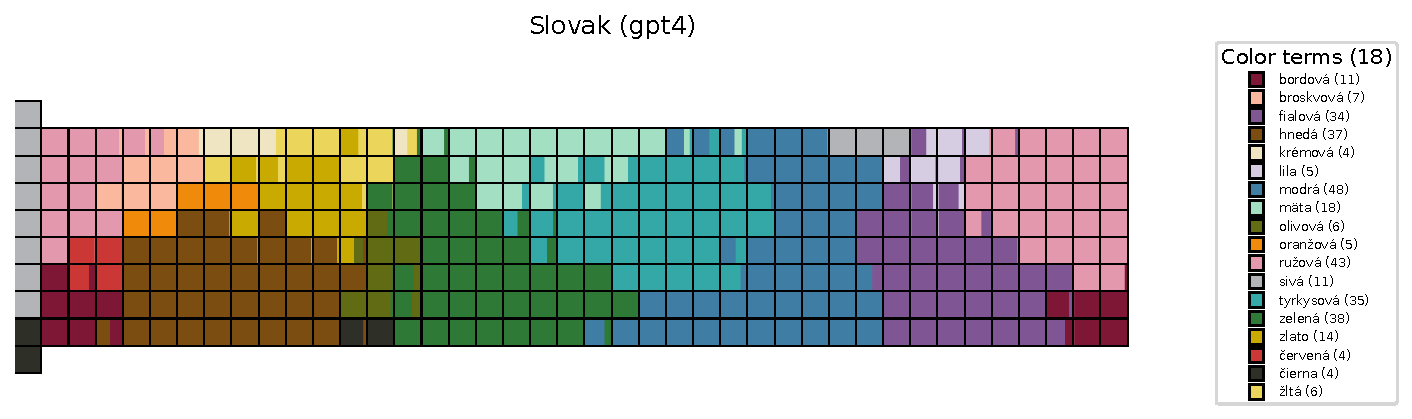
\includegraphics[width=0.49\linewidth]{images/mode_maps_gpt4/Slovak (gpt4).pdf}
\hfill
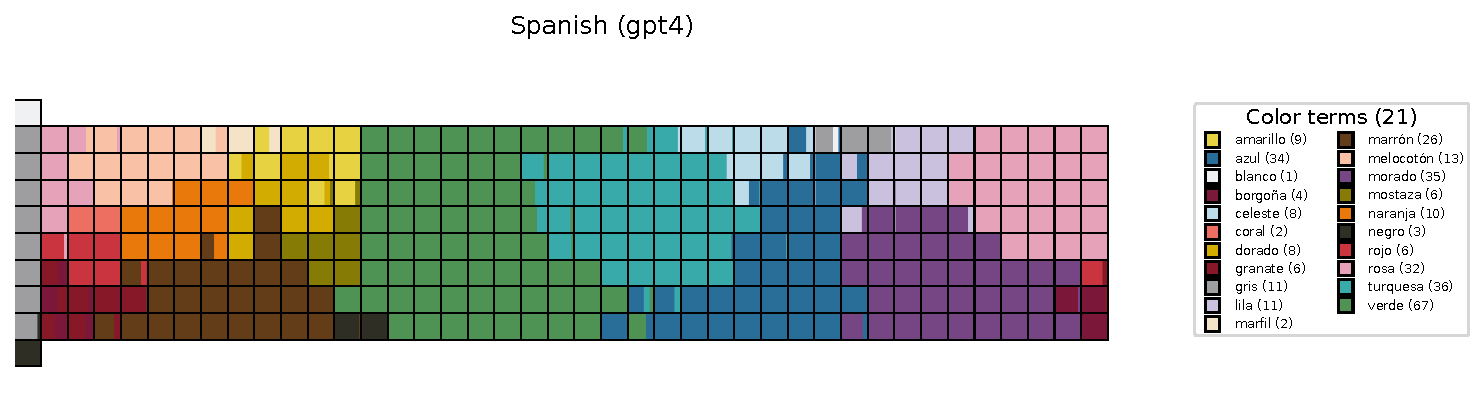
\includegraphics[width=0.49\linewidth]{images/mode_maps_gpt4/Spanish (gpt4).pdf}
\caption[GPT4 Proportion Plots]{GPT4 Proportion Plots}
\label{fig:mode-maps-gpt1}
\end{figure}


\begin{figure}[h!t]
\centering
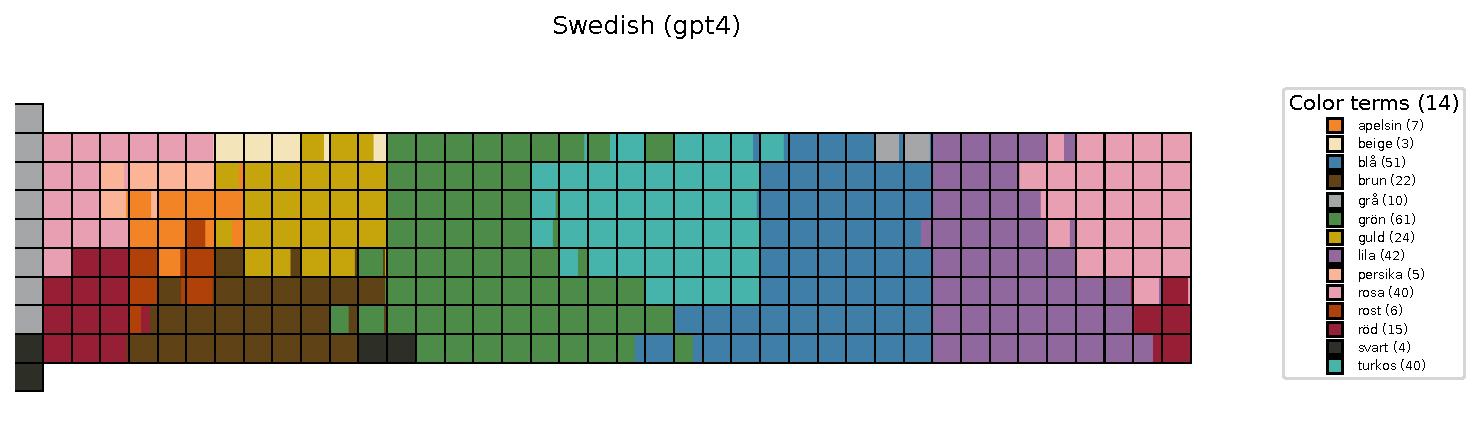
\includegraphics[width=0.49\linewidth]{images/mode_maps_gpt4/Swedish (gpt4).pdf}
\hfill
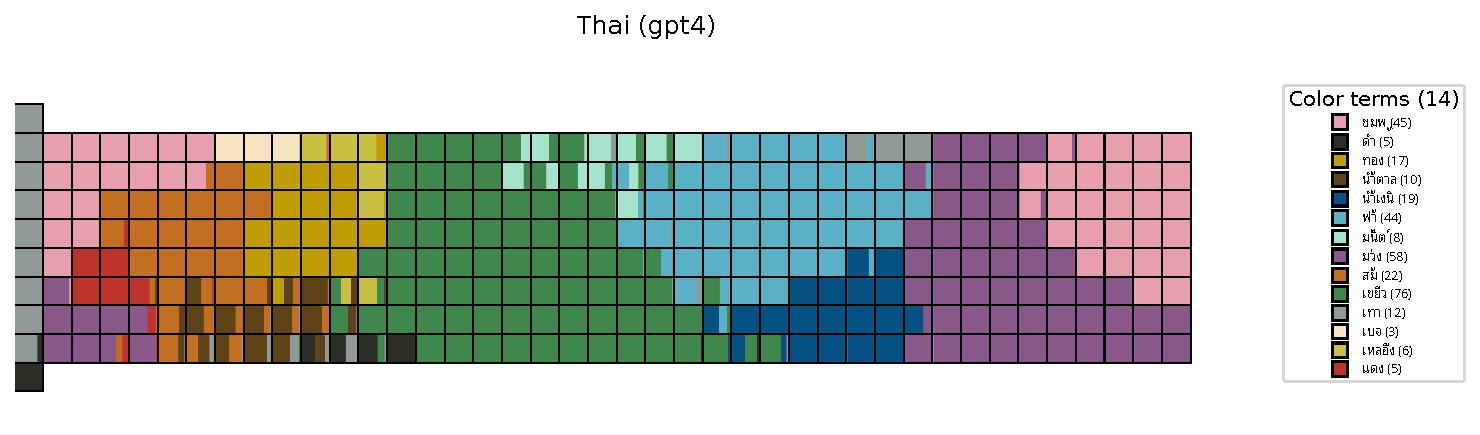
\includegraphics[width=0.49\linewidth]{images/mode_maps_gpt4/Thai (gpt4).pdf}
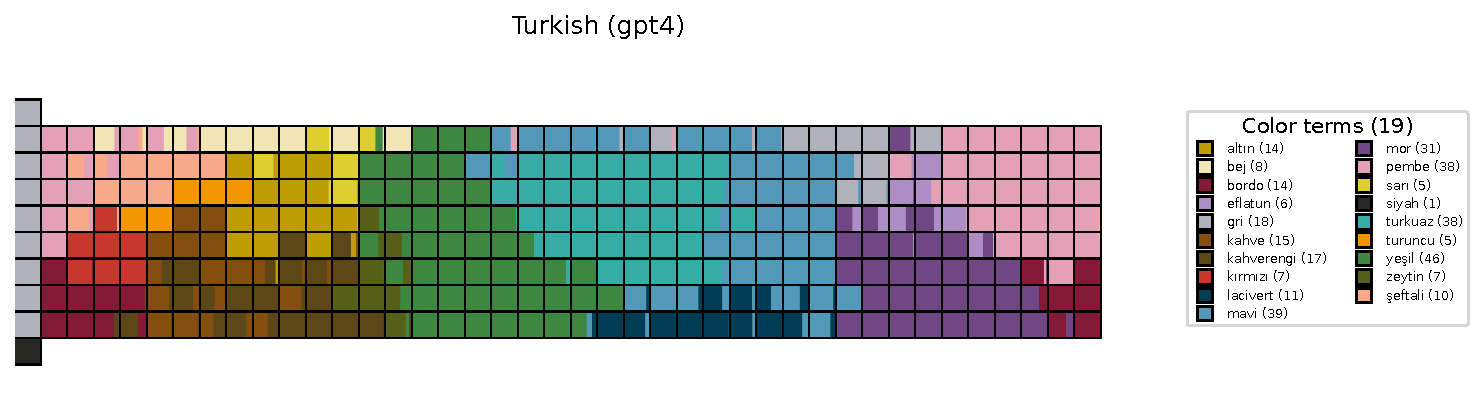
\includegraphics[width=0.49\linewidth]{images/mode_maps_gpt4/Turkish (gpt4).pdf}
\hfill
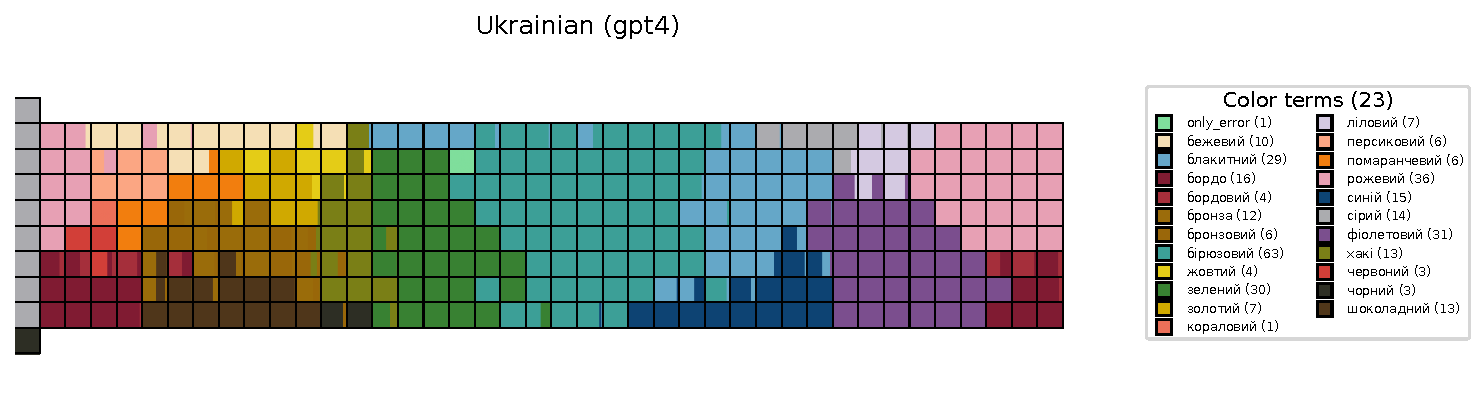
\includegraphics[width=0.49\linewidth]{images/mode_maps_gpt4/Ukrainian (gpt4).pdf}
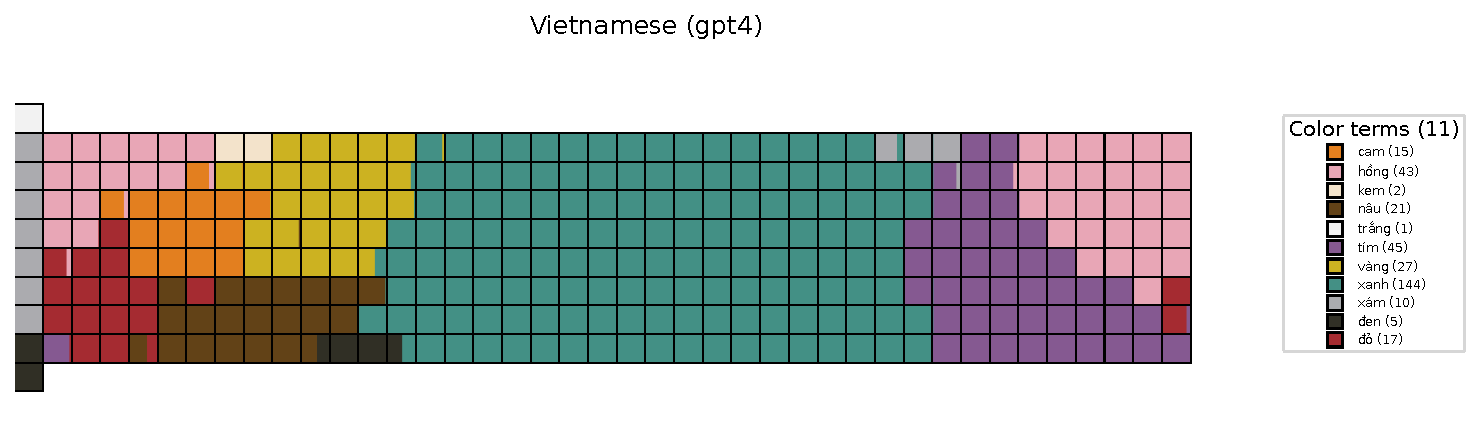
\includegraphics[width=0.49\linewidth]{images/mode_maps_gpt4/Vietnamese (gpt4).pdf}
\caption[GPT4 Proportion Plots]{GPT4 Proportion Plots}
\label{fig:mode-maps-gpt2}
\end{figure}